%%%%%%%%%%%%%%%%%%%%%%%% Chapter 2: Related Work %%%%%%%%%%%%%%%%%%%%
%%%%%%%%%%%%%%%%%%%%%%%%%%%%%%%%%%%%%%%%%%%%%%%%%%%%%%%%%%%%%%%%%%%
\chapter{Related Work}
\label{chapter:related_work}
Continuing from the previous chapter, where we discussed this thesis's goals and their relevance to real-world applications, this chapter provides a detailed literature review of existing distraction detection methods in computer vision. It highlights the limitations of traditional supervised learning methods and underscores the need for innovative unsupervised or self-supervised learning models. Additionally, this chapter addresses research gaps and discusses practical issues associated with the \gls{daa} dataset.

%%%%%%%%%%%%% My Text Here %%%%%%%%%%
\section{Supervised Learning Based Methods}
Supervised learning is a prevalent approach in detecting driver distractions, leveraging annotated datasets to
train models to recognize distraction patterns. In the research work on driver distraction detection,~\citet{58_MIM_zhang2016apply} applied and compared the performance of \gls{svm}~\citep{SVM_cortes1995support} and \gls{cnn}~\citep{CNN_o2015introduction} algorithms using the \gls{sf}~\citep{statefarm2016} dataset which contains 10 classes for driver distraction detection. For \gls{svm}~\citep{SVM_cortes1995support},~\citet{58_MIM_zhang2016apply} utilized a Support Vector Classifier (SVC) model employing a one-vs-one scheme to handle multi-class classification. The \gls{cnn}~\citep{CNN_o2015introduction} approach involved three models: a simple \gls{cnn} based on the MNIST~\citep{MNIST_dataset_deng2012mnist} digit classification task, a transfer learning model leveraging the pre-trained VGG-16~\citep{VGG_16_simonyan2014very}, and a modified VGG model (VGG-GAP)~\citep{VGG_GAP_zhou2016learning} with global average pooling layers. The \gls{cnn} models outperformed the \gls{svm}, with the simple \gls{cnn}~\citep{CNN_o2015introduction} achieving an accuracy of 63.3\%, VGG-16~\citep{VGG_16_simonyan2014very} reaching 90.2\%, and VGG-GAP~\citep{VGG_GAP_zhou2016learning} achieving 91.3\%. The ensemble of VGG-16 and VGG-GAP demonstrated superior performance with an accuracy of 92.6\%~\citep{58_MIM_zhang2016apply}.

\citet{mim_55_alexnet_okon2017detecting} used the AlexNet~\citep{Alexnet_krizhevsky2012imagenet} architecture as a baseline model (Model A) for the driver distraction detection task on the \gls{sf} dataset~\citep{statefarm2016}. AlexNet~\citep{Alexnet_krizhevsky2012imagenet}  was chosen because of its demonstrated capacity to classify a variety of items, including phones and driver's hands, which are useful for detecting distracted driving behaviors. Model A achieved a classification test accuracy of 96.8\% on the \gls{sf} dataset~\citep{statefarm2016}. To increase the model's performance even more,~\citet{mim_55_alexnet_okon2017detecting} introduced an upgraded version (Model B) that incorporated triplet loss. This approach considerably improved classification accuracy, with Model B scoring 98.7\% on the \gls{sf} dataset\citep{mim_55_alexnet_okon2017detecting}.

\citet{59_MIM_Sup_majdi2018drive} proposed `Drive-Net' a supervised learning method that combines a \gls{cnn}~\citep{CNN_o2015introduction} with a random decision forest~\citep{Random_decision_forest_ho1995random} for driver distraction detection.~Drive-Net's~\citep{59_MIM_Sup_majdi2018drive} \gls{cnn} architecture is derived from a modified U-Net~\citep{U_net_ronneberger2015u} model, where the up-convolution layers and the last two down-sampling layers are replaced by a 1x1 convolution layer. The random decision forest~\citep{Random_forest_ferns_bosch2007image} in Drive-Net comprises multiple decision trees trained with randomized data subsets and optimized by maximizing information gain at each node. Drive-Net was evaluated against a \gls{rnn}~\citep{RNN_Used_Object_Rec_liang2015recurrent} and a \gls{mlp}~\citep{MLP_classifier_haykin2009neural} using the \gls{sf} dataset~\citep{statefarm2016}. Utilizing k=5 in k-fold cross-validation~\citep{cross_val_hastie2009elements}, Drive-Net achieved a 95\% classification accuracy, outperforming \gls{rnn} and \gls{mlp} classifiers, which scored 91.7\% and 82\%, respectively\citep{59_MIM_Sup_majdi2018drive}.

\citet{60_MIM_Sup_janet2020real} used \gls{cnn} to detect driver distractions using the \gls{sf} dataset. \citet{60_MIM_Sup_janet2020real} tested three models: a vanilla CNN, a vanilla CNN with data augmentation, and a \gls{cnn} with transfer learning. The vanilla CNN, which included three convolutional layers and three dense layers, had the highest accuracy of 97.66\%. The data-augmented vanilla CNN achieved an accuracy of 97.05\%, while the transfer learning model, which used VGG~\citep{VGG_16_simonyan2014very} and MobileNet~\citep{MobileNet_howard2017mobilenets} to shorten training time, achieved 71.72\%~\citep{60_MIM_Sup_janet2020real}.

\citet{61_MIM_Sup_dhakate2020distracted} introduced an ensemble of \gls{cnn} for driver distraction detection on the \gls{sf} dataset. The proposed approach entails training several \gls{cnn} models, including VGG-16, VGG-19~\citep{VGG_16_simonyan2014very}, InceptionV3~\citep{Inception_V3_szegedy2016rethinking}, ResNet-50~\citep{Resnet_50_he2016deep}, and Xception~\citep{Xception_chollet2017xception}, by eliminating their final layers to extract feature vectors. These vectors are then combined using a stacking ensemble technique to train a meta-classifier \gls{cnn}, achieving a classification accuracy of 97\%. The ensemble stacking technique blends the outputs of different base-level models, enhancing overall prediction accuracy. The best-performing ensemble model in \citep{61_MIM_Sup_dhakate2020distracted} , a combination of ResNet-50~\citep{Resnet_50_he2016deep}, Xception~\citep{Xception_chollet2017xception}, InceptionV3~\citep{Inception_V3_szegedy2016rethinking}, and VGG-19~\citep{VGG_16_simonyan2014very}, achieved 97\% accuracy, significantly outperforming a simpler ensemble model of Xception and InceptionV3, which achieved 73\% accuracy on the \gls{sf} dataset~\citep{61_MIM_Sup_dhakate2020distracted}.

\citet{56_MIM_HCF_9113267} developed a hybrid \gls{cnn} framework (HCF) aimed at detecting distracted driving behaviors on the \gls{sf} dataset. This framework integrated three pretrained models—ResNet50, Inception V3, and Xception—to extract comprehensive behavior features through cooperative transfer learning. The extracted features were integrated into a detailed feature set, which is then classified using fully connected layers.~\citet{56_MIM_HCF_9113267} employed an improved dropout algorithm to prevent overfitting and class activation mapping (CAM) to highlight key features. HCF framework achieved a classification accuracy of 96.74\% on the \gls{sf} dataset~\citep{56_MIM_HCF_9113267}. 

\citet{26_MIM_qin2021distracted} proposed D-HCNN, a \gls{cnn} with decreasing filter fize, for real-time distracted driving detection. \citet{26_MIM_qin2021distracted} focused on building a highly accurate, fast, and low parameter count based model. As a result,  D-HCNN uses only 0.76M parameters, and incorporates Histogram of Oriented Gradients (HOG)~\citep{HOG_dalal2005histograms} images, L2 regularization, dropout, and batch normalization. D-HCNN begins with large convolution filters to capture broad features and progressively reduces filter sizes for detailed feature extraction. The D-HCNN architecture includes four convolutional layers with decreasing filter sizes (12x12, 9x9, 6x6, 3x3), followed by ReLU~\citep{ReLU_DBLP:journals/corr/abs-1803-08375}, max-pooling~\citep{Max_Pooling_32}, batch normalization~\citep{Batch_Norm_DBLP:journals/corr/IoffeS15}, and dropout layers~\citep{dropout_srivastava2014dropout}, concluding with global average pooling~\citep{Global_avg_pooling_Lin2013NetworkIN} and softmax classification. \citet{26_MIM_qin2021distracted} converts RGB images to grayscale in the proposed D-HCNN model to mitigate lighting effects and reduce computation. It also employs zero-mean normalization and random cropping for data augmentation. Evaluated on the AUC Distracted Driver (AUCD2)~\citep{AUC_D3_dataset_abouelnaga2017real} and \gls{sf} datasets, D-HCNN achieved accuracies of 95.59\% and 99.87\%, respectively.

\citet{57_MIM_octave_CNN_9457109} introduced ``OLCMNet" a lightweight octave-like \gls{cnn}~\citep{octave_convolution_chen2019drop}, for detecting driver distraction.~\citet{57_MIM_octave_CNN_9457109} developed an octave-like convolution mixed block (OLCM) to efficiently process feature maps by separating them into low and high-frequency branches, followed by global information fusion through squeeze-and-excitation (SE)~\citep{SE_module_hu2018squeeze} modules.~The architecture consists of a head, feature extraction, and final stage, with the OLCM block reducing spatial redundancy and improving computational efficiency. ~\citet{57_MIM_octave_CNN_9457109} also created Lilong Distracted Driving Behavior (LDDB) dataset, containing 267,378 annotated images from on-road experiments. The proposed OLCMNet achieved 95.98\% accuracy when evaluated on the (LDDB) dataset and 89.53\% accuracy on the \gls{sf} dataset.~\citet{57_MIM_octave_CNN_9457109} highlighted that squeeze-and-excitation module~\citep{SE_module_hu2018squeeze} in the final stage enhanced information exchange between layers, resulting in higher classification accuracy.

The aforementioned research demonstrates the effectiveness of various supervised learning techniques and \gls{cnn} structures, including simple CNNs, transfer learning models, hybrid frameworks, and ensemble methods, in accurately detecting driver distractions on conventional datasets such as \gls{sf} and AUCD2~\citep{AUC_D3_dataset_abouelnaga2017real}. However, there are notable drawbacks linked to using supervised learning methods for the driver distraction detection task. 

\paragraph{Drawbacks of Supervised Learning Based Methods:}
The aforementioned research typically employs supervised \gls{cnn} models, which demand large amounts of labeled data for training. This labeling process is resource-intensive, making it difficult to implement such models in real-world applications. Also these methods rely on manually selected features combined with classifiers and suffer from non-universality and poor adaptability to diverse driving scenarios~\citep{bing_li_2022new, masked_image_modeling_dd_zhang2023novel}. The reliance on supervised frameworks, such as \gls{cnn}s, limits their ability to generalize across different driving scenarios due to the need for extensive reliable labeled data. Furthermore, while \gls{cnn}s are effective at learning local image features, they struggle with capturing the global context necessary for accurately detecting driver distractions in complex real-world environments~\citep{bing_li_2022new, masked_image_modeling_dd_zhang2023novel}. This narrow focus hinders their overall perceptual ability, which is essential for comprehending spatial relationships and high-level semantic information in driving scenes~\citep{masked_image_modeling_dd_zhang2023novel}. Additionally, the intricate nature of real-world driving situations complicates the accurate labeling of data, thereby escalating the difficulty and cost of dataset creation . Overall, these factors contribute to the limited generalization performance and weak iterative ability of current supervised CNN-based models~\citep{masked_image_modeling_dd_zhang2023novel}.

\section{Unsupervised and Self-Supervised Learning Based Methods}
This section presents solutions to the constraints of methods that rely on supervised learning and highlights the advantages of unsupervised and self-supervised learning techniques for detecting driver distraction.~\citet{bing_li_2022new} introduced a novel unsupervised deep learning technique called ``Unsupervised deep learning framework (UDL)" to address the constraints of current supervised methods in driver distraction detection. UDL harnesses vast quantities of unannotated data, hence increasing its applicability for industrial purposes~\citep{bing_li_2022new}. In order to enhance generalization, the Simsiam~\citep{Simsiam_chen2021exploring_stop_grad} unsupervised model was updated.~\citet{bing_li_2022new} incorporated a \gls{mlp} design influenced by RepMLP~\citep{RepMLP_ding2021repmlp}. This architecture combines both local and global feature extraction methods. This method improved the model's capacity to adjust to different driving situations.~\citet{bing_li_2022new} also incorporated residuals into the projection head as a means of mitigating feature deterioration in multilayer architectures. This enhances the process of extracting deep features and improves the precision of detecting distractions~\citep{bing_li_2022new}. A novel loss function was developed by integrating comparative learning~\citep{comparative_learning_chen2020simple} with the stop-gradient~\citep{Simsiam_chen2021exploring_stop_grad} technique. This loss function aims to improve the model's ability to learn robust features, hence boosting its generalization performance~\citep{bing_li_2022new}. The UDL technique underwent testing using the \gls{sf} dataset, and it achieved a notable accuracy rate of 97.38\% during linear evaluation. This performance surpassed that of other unsupervised models like SimSiam with ResNet50 backbone (86.29\%), and SimCLR~\citep{Simsiam_chen2021exploring_stop_grad} with ResNet50 (94.32\%) during linear evaluation~\citep{bing_li_2022new}. The UDL method offers a substantial improvement in identifying driver distraction by utilizing unsupervised learning. The approach optimizes the utilization of unlabeled data, enhances the process of extracting features, and exhibits exceptional performance and flexibility, effectively overcoming the constraints of supervised models~\citep{bing_li_2022new}.

Self-supervised models outperform supervised models in capturing high-level semantic information by focusing feature attention on important discrimination regions more efficiently~\citep{masked_image_modeling_dd_zhang2023novel}.~\citet{masked_image_modeling_dd_zhang2023novel} developed SL-DDBD, a self-supervised learning method for detecting driver distraction behavior. The method uses a masked image modeling framework to reduce labeling costs.~\citet{masked_image_modeling_dd_zhang2023novel} reconfigured the Swin Transformer~\citep{swin_transformer_paper_liu2021swin} encoder, and utilized data augmentation strategies and optimal random masking strategies in the SL-DDBD method. The method achieved 99.60\% accuracy on the \gls{sf} dataset~\citep{statefarm2016}, with pre-training and transfer learning for downstream driver distraction task.

Despite the numerous advantages of unsupervised learning and self-supervised learning over supervised learning, there have been limited research that have applied these methods for identifying driver distraction. Therefore, it is imperative to transition towards these learning paradigms in order to develop more resilient, dependable, and effective systems for detecting driver distraction.

\section{Different Data Modalities}
The success of machine learning models is significantly determined by the quality and characteristics of the data. Similarly, the reliability of driver distraction detection systems relies on the integration of several data modalities and their relationship, as well as their collective impact on overall effectiveness~\citep{RA_2023_dd_article}. Several academics have examined driver distraction detection using various perspectives of data modalities. Physiological data offer direct insights into the driver's condition and correlate strongly with distraction levels~\citep{RA_52_reimer2011impact,RA_89_son2021effects, RA_133_almahasneh2014deep, RA_134_lin2011eeg}. Visual data, crucial for the success of supervised algorithms, includes tracking eye movement and body posture. The precision of these models depends on the accuracy of data collection methods like electroencephalography (EEG), which require adjustments to reduce interference from external physiological activities~\citep{RA_144_lin2005eeg, RA_145_lakshmi2014survey}.~\citet{RA_2023_dd_article} provided an overview of various types of data used in driver distraction detection research. These include physiological data (such as brain activity, breathing rate, skin conductivity and heart rate) and visual data (such as eye movement, body movement, and head movement). \citet{RA_2023_dd_article} emphasized the importance of combining different data modalities to improve the accuracy and reliability of driver distraction detection models. 

\section{Role of Drive and Act Dataset:}
The availability and quality of datasets are critical in exploring solutions to driver distraction.~\citet{moslemi2021computer} summarized the research on driver distraction based on key datasets such as the ~\gls{sf}~\citep{statefarm2016}, and the American University in Cairo (AUC)~\citep{AUC_D3_dataset_abouelnaga2017real} datasets. These datasets vary in characteristics, presenting challenges like differing lighting conditions, camera angles, and the level of detail in recorded actions, which can affect the models' general applicability and effectiveness~\citep{moslemi2021computer}.

The~\gls{daa} dataset, as detailed in~\citep{martin2019drive_and_act_2019_iccv}, is an innovative resource carefully assembled to advance research in driver behavior detection during both manual and automated driving scenarios. This extensive dataset comprises over 9.6 million frames, encapsulating 12 hours of video footage. It systematically captures a broad spectrum of distracting behaviors by integrating diverse types of data such as color, depth, infrared, and 3D body pose information, as illustrated in Figure~\ref{fig:driveandact_salient_features}. Data collection employed six different camera angles, utilizing five Near-Infrared (NIR) cameras and one Kinect v2 camera, the latter used for capturing color images in three channels (RGB), as well as infrared and depth data. The NIR cameras in the dataset operate at a resolution of 1280 x 1024 pixels and a frame rate of 30 Hz, while the Microsoft Kinect camera records color videos at 950 x 540 pixels with a 15 Hz frame rate and captures infrared and depth data at 512 x 424 pixels at 30 Hz~\citep{martin2019drive_and_act_2019_iccv}. The dataset was acquired using a stationary driving simulator, which was selected to ensure participant safety and effectively simulate various driving scenarios. This controlled environment mitigates risks associated with real-world driving and allows for consistent data collection across diverse conditions. Furthermore, the dataset benefits from including a heterogeneous group of participants varying in body size, driving experience, and familiarity with car automation technologies~\citep{martin2019drive_and_act_2019_iccv}. This diversity enriches the dataset, capturing various driving behaviors and styles. The \gls{daa} dataset is randomly segmented into three groups based on the identity of the driver. This splitting approach ensures that data from the same individual is not present across multiple splits, preventing potential overfitting or data leakage~\citet{martin2019drive_and_act_2019_iccv}. Specifically,~\citet{martin2019drive_and_act_2019_iccv} state:

\begin{quote}``for each split, we use the data of ten different identities for training, two for validation, and three for testing." ~\citep{martin2019drive_and_act_2019_iccv}   
\end{quote}

By splitting the dataset in this manner, the authors aim to create a challenging benchmark that evaluates the generalization capabilities of models trained on the \gls{daa} dataset. The three distinct splits allow for proper training, validation, and testing procedures, enabling robust evaluation of driver behavior recognition and driver distraction detection algorithms on unseen data from new individuals not present in the training set.

The \gls{daa} dataset uses a three-level hierarchy to detail driver interactions as depicted in the figures~\ref{fig:driveandact_activities} and~\ref{fig:driveandact_salient_features}, providing a comprehensive framework for analyzing driver behavior under both manual and automated conditions. At the highest level of the hierarchy are the tasks, which outline broad scenarios that participants encountered during the data collection. These tasks, such as entering the car and switching to autonomous driving, set the context for the actions and are vital for simulating realistic driving environments. They also include potentially distracting situations anticipated with increased automation, like using a laptop. The mid-level in this hierarchy consists of mid-level actions. These are fine-grained activities that further break down the tasks into more specific behaviors but still maintain a clear semantic meaning. For example, while a task might involve using a laptop, the mid-level actions detail the individual activities involved, such as typing or browsing. At the most detailed level are atomic action units, which describe basic interactions within the driving environment without long-term semantic implications. These units are defined by a combination of action, object, and location—such as `reaching for a jacket in the left backseat'. This level provides the fundamental building blocks of driver behavior, capturing the minute detail of every interaction~\citep{martin2019drive_and_act_2019_iccv}.

This hierarchical labeling not only enhances the granularity of behavioral analysis but also supports the development of sophisticated models that can predict and interpret diverse driving behaviors in real-time. By examining these interactions across different levels of abstraction, researchers can gain deeper insights into how drivers respond to various driving conditions and tasks, contributing to safer automotive technologies.

\begin{figure}[htbp]
\begin{center}
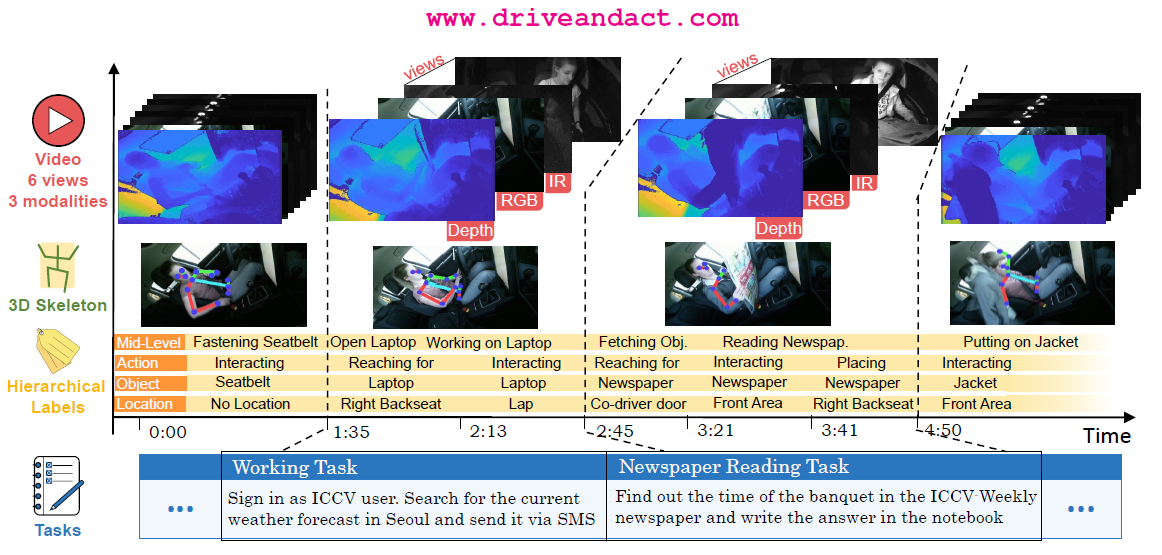
\includegraphics[width=0.8\textwidth]{Images_Thesis/daa_images/Capture_daa_thesis.PNG}
\end{center}
\caption[Drive and act dataset with its salient features.]{Drive and act dataset with its salient features. On the y-axis different modalities in the drive and act dataset can be seen along with the hierarchical labeling scheme guided by the 12 predefined tasks that each participant is subjected to perform in order to do the desired data collection. On the x-axis the time stamps along with the tasks that each participant in performing with respect to the time is shown. This figure also depicts the hierarchy in labeling where mid-level activities are fine grained activities and action, object and location combined together forms a complete driver action. Source:~\citep{martin2019drive_and_act_2019_iccv}.}
\label{fig:driveandact_salient_features}
\end{figure}

\subsection{Advantages of the Drive and Act Dataset:}
The \gls{daa} dataset provides different modalities, i.e., Color, Infra-Red, Depth and 3D skeleton data, which can be combined with each other to develop complex and reliable driver distraction detection systems. Given the imbalanced nature of the \gls{daa} video dataset,~\citet{martin2019drive_and_act_2019_iccv} segmented the \gls{daa} dataset into three distinct partitions: Split 0, Split 1, and Split 2. They advocated for the training, evaluating, and testing deep learning models across these three splits. They recommended that the resultant metrics, such as balanced accuracy~\citep{bal_acc_paper_brodersen2010balanced}, be averaged to yield a statistically robust performance measure. This approach is a proposed remedy to counter the dataset's imbalance. This method of dataset division can be effectively integrated with additional strategies to further mitigate the imbalance in the \gls{daa} dataset~\citep{martin2019drive_and_act_2019_iccv}. This approach facilitates robust model evaluation across different data segments, ensuring statistical reliability in our findings. 

\begin{figure}[h]
\begin{center}
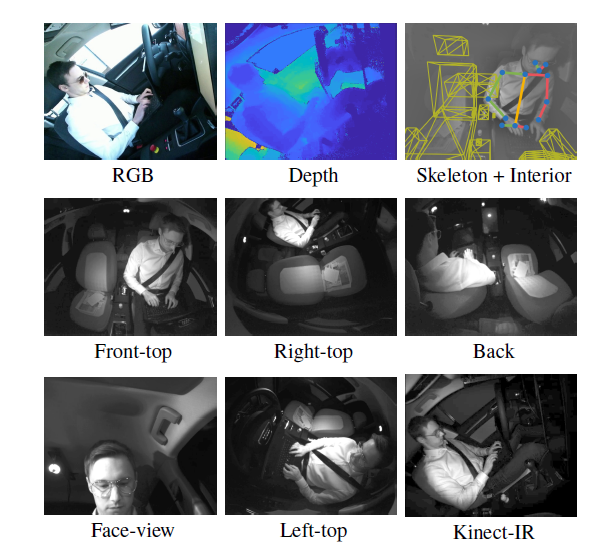
\includegraphics[width=0.8\textwidth]{Images_Thesis/daa_images/Capture_views_thesis.PNG}
\end{center}
\caption[Illustrative images depicting the action of working on a laptop from various views and using different modalities.]{Illustrative images depicting the action of working on a laptop from various views and using different modalities. Source:~\citep{martin2019drive_and_act_2019_iccv}.}
\label{fig:driveandact_views_modalities}
\end{figure}

\subsection{Challenges of the Drive and Act Dataset}
\label{section:Disadvantages of Drive and Act Dataset}
The distribution of all 83 driver actions provided by the \gls{daa} video dataset is depicted in figure~\ref{fig:driveandact_activities}. Each activity is captured for a duration of 3 seconds in one video sample~\citep{martin2019drive_and_act_2019_iccv}. In the figure~\ref{fig:driveandact_activities}, the y-axis depicts the frequency of each activity, while the x-axis represents the 83 activities. It is evident from the figure ~\ref{fig:driveandact_activities} that an important obstacle in the \gls{daa} video dataset is the unequal distribution of classes among all 83 activities including the 34 fine-grained activities~\citep{martin2019drive_and_act_2019_iccv}. This disparity is a substantial obstacle for creating models that can effectively identify rare but potentially vital driving behaviors.~It is crucial to address this issue in order to develop strong models that can accurately detect a variety of actions, including some that are less frequent but may have greater potential for harm. 

\begin{figure}[h]
\begin{center}
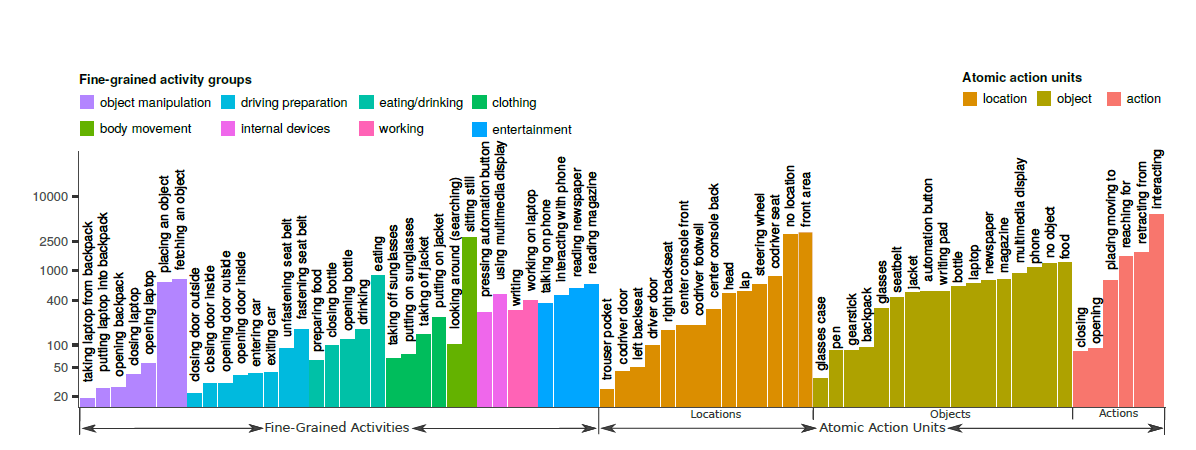
\includegraphics[width=0.8\textwidth]{Images_Thesis/daa_images/Capture_Activities_thesis.PNG}
\end{center}
\caption[Distribution of activities offered by Drive and Act video dataset.]{Distribution of Activities in the Drive and Act Video Dataset. The x-axis represents fine-grained activities, followed by atomic action units, while the y-axis shows the number of video samples, ranging from 0 to 10,000. Source:~\citep{martin2019drive_and_act_2019_iccv}.}
\label{fig:driveandact_activities}
\end{figure}

\subsection{Comparing Drive and Act to Other Datasets}
The \gls{daa} dataset~\citep{martin2019drive_and_act_2019_iccv} is distinguished from current datasets such as NTU~\citep{DBLP:journals/corr/NTUShahroudyLNW16}, HEH~\citep{HEHOhnBar2014HandGR}, AUC~\citep{DBLP:journals/corr/AUCDDAbouelnagaEM17} and Kinetics~\citep{DBLP:journals/corr/KineticsCarreiraZ17} by its large size, wide range of activities recorded, and inclusion of both manual and automated driving situations for Action Recognition. 
For example, the AUC dataset~\citep{DBLP:journals/corr/AUCDDAbouelnagaEM17} contains only 17,000 images, and the NTU dataset~\citep{DBLP:journals/corr/NTUShahroudyLNW16} contains 4 million images, both of which are significantly smaller than the over 9.6 million images provided by the DAA dataset. The Kinetics~\citep{DBLP:journals/corr/KineticsCarreiraZ17} contains more than 76 million images and is exception in terms of size, however it only offers one camera view compared to 6 camera views in \gls{daa} dataset. This comprehensive approach distinguishes it as a significant resource for the research community and highlights its potential to promote breakthroughs in driver behavior identification systems. However, there is an urgent requirement for creative solutions to address the issues of class imbalance and to efficiently utilize the dataset's multi-modal and multi-view data. This dataset provides unparalleled opportunity for researchers in a broad range of domains, particularly in tackling the issue of imbalanced datasets. It enables the \gls{daa} dataset to be bench-marked against the most recent models in a variety of domains, including multi-class and binary classification, view and modality generalization, and the creation of hybrid approaches that use multi-modal technology. These cutting-edge technologies are essential for driver distraction detection, behavior tracking, and the creation of intelligent perceptual user interfaces. By leveraging cutting-edge technology across multiple modalities, this dataset sets the path for major developments in understanding and increasing driver safety and interaction.

In this thesis, we focus on two data modalities from the \gls{daa} dataset: Color and Infrared. An illustration of these modalities, as seen in the action of working on a laptop, is shown in Figure~\ref{fig:driveandact_views_modalities}. The \gls{daa} dataset, derived from video captured with Kinect and NIR cameras, serves as the source of video data for this research. The transformation of this video data into image data is accomplished by extracting frames, a process guided by the dataset's annotation files across all splits. This thesis explores the challenges posed by the significant class imbalance found within these image datasets, a phenomenon that is often extrinsic~\citet{5128907Haibo_Imbalance}. For example, categorizing actions from the \gls{daa} dataset into distracted versus non-distracted classes introduces an inherent imbalance due to varying sample sizes across the 34 fine-grained classes present in the mid-level hierarchical labeling of the \gls{daa} dataset, and can be seen in the figure~\ref{fig:driveandact_activities}. Chapter~\ref{chapter:proposed_methods} provides a detailed analysis of the image datasets and tackle the difficulties caused by imbalanced datasets by proposing and explaining the `Clustered Feature Weighting' algorithm.

\subsection{Key Challenges Posed by Imbalanced Datasets}
Researchers such as~\citep{5128907Haibo_Imbalance, Survey_DL_Taghi_article}, summarised the key challenges posed by imbalanced datasets as follows:
\begin{itemize}
    \item \textbf{Model Bias:} Models trained on imbalanced data typically exhibit a bias towards the majority class, leading to insufficient representation and prediction of minority classes~\citep{imbalance_kC_rawat2022review, 5128907Haibo_Imbalance}.
    \item \textbf{Poor Generalization:} Models may generalize poorly on new, unseen data, especially for under-represented classes~\citep{5128907Haibo_Imbalance, Survey_DL_Taghi_article}.
    \item \textbf{Evaluation Challenges:} Conventional accuracy measurements can be false as they may primarily indicate the frequency of the dominant category rather than the actual prediction capacity of the model in various situations~\citep{5128907Haibo_Imbalance, Survey_DL_Taghi_article}.
\end{itemize}

\section{Existing Solutions to Imbalanced Datasets}
In machine learning, deep learning, and computer vision, learning from datasets that are imbalanced has become a major problem that makes it hard to get high-performance algorithmic results. An imbalanced dataset is characterized by an unequal distribution of classes, a topic that has been extensively explored in the existing literature~\citep{Fernndez2018LearningFI}, ~\citep{5128907Haibo_Imbalance}. This imbalance can develop either organically, as a result of the inherent differences in the frequency of data occurrence, as shown in medical diagnostics, or extrinsically, due to external factors such as the methods used to collect data~\citep{articleSurveyImData},~\citep{5128907Haibo_Imbalance}). According to~\citet{articleKrawczyk}, it is possible to achieve appropriate outcomes regardless of class imbalance, as long as both classes for example in binary classification are sufficiently represented and come from separate distributions~\citep{articleSurveyImData}.

Within the field of image classification, extensive study has been conducted on the issue of imbalance in both binary and multi-class frameworks, resulting in the development of numerous strategies for reducing imbalance problems~\citep{5128907Haibo_Imbalance,H_13_chawla2002smote,H_44_han2005borderline,H_45_he2008adasyn}. However, the usefulness of these strategies varies depending on the application instance, with each approach having its own set of advantages and drawbacks. Traditionally, research has concentrated mostly on machine learning models~\citep{H_75_akbani2004applying, H_77_vilarino2005experiments, H_78_kang2006eus, H_81_tang2006granular}. Nonetheless, current advances in the field of computer vision, natural language processing~\citep{NLP_chen2021multi} and deep learning need a move toward investigating how deep learning models can tackle data imbalance problems or how efficient they are when exposed to imbalanced data~\citep{articleSurveyImData}. According to~\citet{articleJapkowicz2systematicstudy}, the severity of the imbalance problem depends on the degree of class imbalance, the complexity of data representation, the volume of training data, and the classification technique used~\citep{AjayDBLP:journals/corr/abs-2108-00071}.
The Imbalance Ratio (ImR) is a metric that measures the degree of class imbalance. It is calculated as the ratio of the number of samples in the majority class to the number of samples in the minority class~\citep{Fernndez2018LearningFI}. With respect to binary image classification, the terms `majority class' or `negative class' refer to the class with the most samples, whereas `minority class' or `positive class' implies the class with the fewest examples~\citep{AjayDBLP:journals/corr/abs-2108-00071}. The same terminology can be transferred to the domain of multi-class image classification problems.

In order to mitigate the consequences of imbalance, a number of measures are outlined in~\citep{Survey_DL_Taghi_article}. The following are the main solutions:
\begin{itemize}
    \item \textbf{Resampling Techniques:} The dataset can be balanced by oversampling minority classes or undersampling majority classes~\citep{5128907Haibo_Imbalance,Survey_DL_Taghi_article}.
    \item \textbf{Evaluation Metrics:} Adoption of metrics such as the balanced accuracy score, precision, recall, F-1 score, and the area under the Receiver Operating Curve (AUC-ROC) provide a more accurate measure of model performance in the context of imbalanced data~\citep{Survey_DL_Taghi_article, 18_wang2016training}.
    \item \textbf{Class Weight Adjustments:} During model training, adjusting class weights compensates for imbalances by assigning greater importance to minority classes within the loss function~\citep{Survey_DL_Taghi_article}.
\end{itemize}


\subsection{Learning from Imbalanced datasets}
The seminal work ``Learning from Imbalanced Data" by~\citet{5128907Haibo_Imbalance} not only offers a thorough examination of the challenges posed by datasets characterized by under-representation and substantial class imbalances, but also provides practical recommendations for addressing these issues. This study elucidates the difficulties conventional machine learning techniques, which are typically designed for balanced class distributions, encounter in the face of pronounced class disparities. It underscores the inadequacy of traditional metrics, such as overall accuracy~\citep{metric_accuracy_grandini2020metrics} or error rate, in accurately evaluating the performance of algorithms in imbalanced learning scenarios.~\citet{5128907Haibo_Imbalance} advocate for the adoption of more sophisticated evaluation methods, such as receiver operating characteristics (ROC) curves~\citep{ROC_intro_fawcett2006introduction}, precision-recall curves~\citep{precision_recall_giglioni2021use}, and cost curves~\citep{precision_recall_giglioni2021use}, which provide a more detailed insight into performance dynamics. Additionally, the paper highlights the challenges posed by relative imbalances—common in real-world settings—and the significant learning obstacles introduced by the scarcity of representative data for rare instances. Importantly, the authors acknowledge the complexity of datasets and relative imbalances as key contributors to the degradation of classification performance, further exacerbated by factors such as within-class imbalances and small disjuncts~\citep{5128907Haibo_Imbalance}. The authors have presented a comprehensive categorization of solutions available for addressing the issue of learning from imbalanced datasets, as depicted in figure~\ref{fig:imb-learn-tech}. They have also provided detailed explanations for each category and method. Additionally, they have offered criticisms of commonly used solutions, such as sampling methods designed to balance datasets. These critiques address the limitations of undersampling and oversampling, such as the possibility of losing important information and the potential for overfitting.~\citet{5128907Haibo_Imbalance} express significant criticism towards the~\gls{smote}~\citep{H_13_chawla2002smote} method, highlighting its vulnerability to overgeneralization and variance issues. Specifically, the~\gls{smote} algorithm's tendency to generate synthetic data without careful consideration, which might unintentionally blur class boundaries or in other words obscure the distinction between different classes as originally highlighted by~\citep{43_wang2004imbalanced}. The blurring of class boundaries poses challenges for models in differentiating between classes due to the potential resemblance or encroachment of synthetic data points onto the data space of the majority class, or the inaccurate representation of the minority class. This could potentially diminish the efficacy of the model, as it may encounter difficulties in appropriately categorizing novel instances that lie in close proximity to these indistinct boundaries~\citep{43_wang2004imbalanced}.


\tikzset{%
    ,parent/.style={align=left,text width=3cm,rounded corners=1pt}
    ,child/.style={align=left,text width=6.7cm,rounded corners=1pt}
    }
   
\begin{figure}[htbp]
    \centering
    \small
    \begin{forest}
        for tree={%
            ,scale=.55
            ,grow'=east
            ,forked edges
            ,draw
            ,rounded corners
            ,node options={align=left}
            ,text width=4cm
            ,anchor=west
            }
        [Imbalanced Learning\\Techniques~\citep{5128907Haibo_Imbalance}, fill=gray!25, parent
            [Sampling Techniques for Imbalanced Learning, tier=align here, 
            for tree={fill=brown!25, child}
                [Random Oversampling and Undersampling]
                [Informed Undersampling
                    [EasyEnsemble $\&$ BalanceCascade\citep{H_40_liu2008exploratory}]
                    [KNN based:(NearMiss-1)~(NearMiss-2)~(NearMiss-3)~(Most Distant)~\citep{H_41_mani2003knn}]
                    [One-sided selection (OSS)~\citep{H_42_kubat1997addressing}]
                ]
                [Synthetic Sampling with Data Generation
                    [\gls{smote}~\citep{H_13_chawla2002smote}]
                ]
                [Adaptive Synthetic Sampling
                    [Borderline-\gls{smote}~\citep{H_44_han2005borderline}]
                    [Adaptive Synthetic Sampling~\citep{H_45_he2008adasyn}]
                ]
                [Sampling with Data Cleaning
                    [Tomek links~\citep{H_46_tomek1976two_4309452}]
                    [OSS method~\citep{H_42_kubat1997addressing}]
                    [Condensed nearest neighbor rule and Tomek Links~\citep{H_22_batista2004study}]
                    [Neighborhood Cleaning Rule~\citep{H_36_laurikkala2001improving}]
                    [\gls{smote} $+$ ENN and \gls{smote} $+$ Tomek~\citep{H_22_batista2004study}]
                ]
                [Cluster-Based Sampling
                    [Cluster-based oversampling~\citep{H_27_jo2004class}]
                ]
                [Integration of Sampling and Boosting
                    [\gls{smote}-Boost~\citep{H_47_chawla2003smoteboost}]
                    [Data-Boost-IM~\citep{H_14_guo2004learning}]
                    [JOUS-Boost~\citep{H_38_mease2007boosted}]
                ]
            ]
            [Cost-Sensitive Approaches, 
            for tree={fill=red!25,child}
                [Cost-Sensitive Learning Framework
                    [Translation theorem~\citep{H_55_zadrozny2003cost}] 
                    [Metacost framework~\citep{H_54_domingos1999metacost}]
                ]
                [Cost-Sensitive Dataspace Weighting with Adaptive Boosting
                    [(AdaC1)~(AdaC2)~(AdaC3)~\citep{H_58_sun2007cost}] 
                    [AdaCost~\citep{H_59_fan1999adacost}]
                ]
                [Cost-Sensitive Decision Trees and Neural Networks]
            ]
            [Kernel-Based Methods, tier=align here, 
            for tree={fill=blue!25, child}
                [Kernel-Based Learning Framework
                    [~\gls{svm}~\citep{H_23_japkowicz2002class}]
                ]
                [Kernel Methods with Sampling
                    [\gls{smote} with Different Costs~\citep{H_75_akbani2004applying}] 
                    [Ensembles of over/undersampled~\gls{svm}~\citep{H_77_vilarino2005experiments}~\citep{H_78_kang2006eus}~\citep{H_79_liu2006boosting}~\citep{H_80_wang2008boosting}] 
                    [Granular \gls{svm}—Repetitive Undersampling~\citep{H_81_tang2006granular}]
                ]
                [Kernel Modification Methods
                    [Kernel classifier construction~\citep{H_85_hong2007kernel}] 
                    [(Boundary movement)~(Biased penalties)~(Class-boundary alignment)~\citep{H_76_wu2003class}] 
                    [Kernel-boundary alignment~\citep{H_86_wu2004aligning}~\citep{H_87_wu2005kba}] 
                    [k-category Proximal \gls{svm} with Newton refinement~\citep{H_91_fung2001proximal}] 
                    [Support cluster machines~\citep{H_92_yuan2006learning}] 
                    [Kernel neural gas for imbalanced clustering~\citep{H_93_qin2004kernel}] 
                    [(P2PKNNC algorithm)~(P2P communication paradigm)~\citep{H_94_yu2007novel}]
                ]
            ]
            [Active Learning Methods, 
            for tree={fill=green!25, child}
                [Simple active learning heuristic~\citep{H_103_doucette2008gp}]
            ]
            [Supplementary Approaches, tier=align here, 
            for tree={fill=orange!25, child}
                [One-class \gls{svm}~\citep{H_74_raskutti2004extreme}] 
                [Autoassociator method~\citep{H_109_japkowicz2001supervised}~\citep{H_110_manevitz2007one}~\citep{H_111_japkowicz2000learning}~\citep{H_112_japkowicz1995novelty}] 
                [Ensemble knowledge for imbalance sample sets (eKISS)~\citep{H_12_tan2003multi}]
            ]
        ]
    \end{forest}
    \caption[Classification of Imbalanced Learning Techniques]{A flow chart showing the classification of Imbalanced Learning Techniques proposed by~\citet{5128907Haibo_Imbalance}.}
    \label{fig:imb-learn-tech} % Label for cross-referencing
\end{figure} 

Additionally,~\citet{Data_algo_hybrid_krawczyk2016learning} categorize the strategies for addressing imbalanced datasets into three principal techniques. Initially, they examine data-level approaches, which involve adjustments to the sampling process either to balance the class distribution or to eliminate problematic samples. The second category encompasses algorithm-level strategies, which modify the core learning algorithms to better manage data with skewed distributions, thereby reducing the bias towards majority class instances~\citep{Data_algo_hybrid_krawczyk2016learning, Fernndez2018LearningFI}. Subsequently,\citet{Data_algo_hybrid_krawczyk2016learning} provide hybrid methods that combine the benefits of both data-level and algorithm-level approaches~\citep{Navo_Im_chakrabarty2020navo}.

\citet{Fernndez2018LearningFI} explored the challenges associated with learning from imbalanced datasets thoroughly in \textit{Learning from Imbalanced Data Sets}~\citep{Fernndez2018LearningFI}. Similarly, \citet{Survey_DL_Taghi_article} provide a detailed review of methods to tackle class imbalance in machine learning, with an emphasis on deep learning techniques. \citet{Survey_DL_Taghi_article} categorizes the various techniques, defines appropriate assessment criteria for imbalanced datasets, and underscores the significance of both supervised and unsupervised learning approaches, including those that incorporate transfer learning. \citet{Survey_DL_Taghi_article} notes that traditional metrics like accuracy can misleadingly reflect performance in imbalanced contexts due to their susceptibility to the prevalence of the majority class~\citep{Fernndez2018LearningFI, Survey_DL_Taghi_article}. Instead, Balanced Accuracy (BA)~\citep{bal_acc_paper_brodersen2010balanced} is recommended as it accounts for both the True Positive Rate (TPR) and the True Negative Rate (TNR), offering a comprehensive measure of model efficacy across both majority and minority classes and mitigating the inherent bias of simpler metrics~\citep{18_wang2016training}. \citet{Survey_DL_Taghi_article} identifies a gap in the exploration of deep learning strategies for managing class imbalance, with most current methods, particularly those involving sampling or algorithmic modifications, falling within the domain of supervised learning due to their reliance on labeled data for adjusting class distributions or refining learning algorithms based on class-specific insights~\citep{Survey_DL_Taghi_article}. The discourse also touches on innovative deep learning techniques such as dynamic sampling, two-phase learning, and enhancements involving novel loss functions and cost-sensitive learning~\citep{Survey_DL_Taghi_article}. Additionally, the integration of transfer learning with deep learning strategies to enhance model performance on imbalanced datasets is discussed. Despite the prevalence of supervised methods, the field of unsupervised learning in relation to class imbalance remains under-explored and represents a promising area for future research.

\subsection{Transfer Learning and Clustering-Based Techniques}
Transfer learning is an advantageous approach in deep learning that can address the problem of class imbalance. By initially training on diverse and wide datasets and then fine-tuning the model on the unbalanced dataset, it is possible to strengthen the model's capacity to generalize its knowledge to new scenarios and enhance its overall performance~\citep{Survey_DL_Taghi_article}. This approach is especially beneficial for classes that have a restricted number of examples, as conventional learning methods may lead to below-average model performance~\citep{Survey_DL_Taghi_article}. The review paper discusses various methods, such as category centers (CC) proposed by~\citet{91_zhang2018image}, Large Margin Local Embedding (LMLE) introduced by~\citet{22_huang2016learning}, and Deep Over Sampling (DOS) developed by~\citet{117_ando2017deep}. These methods utilize hybrid approaches that combine transfer learning, deep feature representations, and k-nearest neighbors to tackle imbalanced datasets~\citep{Survey_DL_Taghi_article}.

Clustering-based methods have become a sophisticated approach to tackle class imbalance by focusing on grouping instances into clusters before applying subsampling methods. This strategy aims to preserve the integrity of information while simultaneously providing a more equitable distribution among different classes~\citep{densitybased_IM_munguia2023density}. More precisely, algorithms such as K-means~\citep{kmeans_kaufman2009finding} and \gls{clara}~\citep{kmeans_kaufman2009finding} aid in the creation of clusters within classes by choosing instances that are both representative and diverse. A significant progress in this field is the utilization of density-based clustering methods, specifically \gls{dbscan}~\citep{DBSCAN_algo_ester1996density} and \gls{hdbscan}~\citep{HDBSCAN_algo_campello2013density}. These algorithms excel at handling datasets with varying sizes, shapes, and densities by detecting regions with high population density. This allows for reducing the size of the majority class without significant loss of information~\citep{densitybased_IM_munguia2023density}.


\citet{densitybased_IM_munguia2023density} makes a comprehensive contribution by presenting a new density-based undersampling technique that exploits the capabilities of \gls{dbscan} and \gls{hdbscan}, in addition to an improved \gls{scut}~\citep{SCUT_agrawal2015scut} algorithm. This approach, when used with imbalanced and multi-class hyperspectral remote sensing images, employs geometric mean values and Friedman's test~\citep{Friedman_Test_7c3c84e5-7230-3033-8b6c-ec430fb73d61} to thoroughly assess its effectiveness. The results emphasize the effectiveness of density-based clustering methods in addressing the difficulties posed by severe class imbalances, representing a notable shift from conventional strategies~\citep{densitybased_IM_munguia2023density}.

~\citet{densitybased_IM_munguia2023density} introduces methodological advancements that suggest a more precise equilibrium between undersampling and oversampling, depending on the average size of each class sample. This strategy effectively combines density-based clustering with the \gls{scut} method to dynamically modify class sizes. It utilizes \gls{dbscan}~\citep{DBSCAN_algo_ester1996density} or \gls{hdbscan}~\citep{HDBSCAN_algo_campello2013density} for classes that are above the average and employs \gls{smote}~\citep{H_13_chawla2002smote} for classes that are below the average. This strategy seeks to achieve both a more equitable representation of classes and improved classifier performance by utilizing geometric mean values as a measure of success. The suggested method effectively addresses the issue of class imbalance by deliberately removing instances from the majority class using density-based clustering and increasing the representation of the minority class through \gls{smote}. The empirical validation of this method, which shows significant improvements in the accuracy of classifying highly unbalanced datasets, highlights the potential of combining density-based clustering with sampling approaches as an effective solution to the challenges caused by class imbalance.

The research by~\citet{densitybased_IM_munguia2023density} contends that conventional oversampling techniques such as \gls{smote} and its variations aim to achieve balance in the dataset, but they may not adequately address the nuances of class imbalance. On the other hand, clustering methods, especially those that rely on density, provide a strong and reliable alternative.

\paragraph{Research Gap:}~The emergence of~\gls{vit} models has had a tremendous impact on the field of computer vision. Despite this advancement, the use of these models to address the common issue of dataset imbalance has not been widely examined. This oversight signifies a crucial research gap, neglecting the potential of \gls{vit} models to serve as general-purpose tools for extracting intricate image features. Vision Transformers are distinguished by their ability to assimilate complex visual representations, which provides access to a rich feature space for developing novel techniques to handle the imbalanced learning challenge. This feature space, strengthened by training on large and diverse image datasets, has a wide range of visual properties. Such a collection of information is useful in finding both tiny differences and similarities between images, presenting a viable solution to the imbalance problem. It offers a thorough understanding and representation of minority classes, which are typically excluded and ignored by standard models. The comprehensive representation offered by \gls{vit} models opens up opportunities for the advancement of sampling strategies, augmentation techniques, and customized loss functions that are particularly crafted to address the distinct difficulties presented by unbalanced datasets. By innovating techniques that exploit the feature space of Vision Transformers~\citep{Vit_Paper_Dosovitskiy2020AnII}, there lies the potential to inaugurate a new phase of progress in deep learning. This advancement is particularly crucial in achieving equitable and consistent model performance across all class categories within imbalanced datasets.


Within the context of this thesis, Chapter~\ref{chapter:proposed_methods} focuses on introducing and explaining such a novel sampling technique called ``ClusteredFeatureWeighting" that combines the effective use of feature space of \gls{vit} using Transfer Learning, Density-Based Clustering, and Weighted Random Sampling. This novel approach is specifically tailored to rectify the imbalance dataset problem inherent in the drive and act dataset~\citep{martin2019drive_and_act_2019_iccv}. Subsequent chapters, particularly Chapters~\ref{chapter:background} and~\ref{chapter:proposed_methods}, provide a comprehensive explanation of the working principles and experimental methodologies. Chapter~\ref{chapter:Experiments and Results} presents the results after each experiment by employing the methodology explained in the chapter~\ref{chapter:proposed_methods}.



